%compile with XeLaTeX
\documentclass[11pt,a4paper,titlepage]{article}
\usepackage[utf8]{inputenc}
\usepackage[german]{babel}
\usepackage[T1]{fontenc}
\usepackage{fontspec}
\setmainfont{Arial}
\usepackage{amsmath}
\usepackage{amsfonts}
\usepackage{amssymb}
\usepackage{graphicx}
\usepackage[onehalfspacing]{setspace}
\usepackage[left=2cm,right=2cm,top=2cm,bottom=2cm]{geometry}
\graphicspath{{./img/}}
\usepackage{titlepic}

\titlepic{
\includegraphics[width=\textwidth]{darwin.png}}

\author{Michael Schaufelberger (Product Owner)\\
Filip Kašiković (Scrum Master)\\
Raphael Mailänder\\
Simon Stucki\\
Berli Marc\\
Ferenc Kuntić}


\title{Projekt Darwin}

\begin{document}

\maketitle

%ZHAW School of Engineering
%IT17ta_ZH
%PSIT 4

\begin{abstract}

%250 wörter
% Einleitung: Definiere Problematik und begründe Revelanz der Untersuchung
In der heutigen Zeit haben sich Videospiele als Teil unserer Gesellschaft stark gefestigt und ein Teil unseres Alltags geworden. Die Wirtschaft und Präsenz der Spieleindustrie wächst vom Jahr zu Jahr stetig an und bildet ein sehr lukratives Geschäftsumfeld. Erträge und Umsätze in Milliardenhöhe sind keine Besonderheit. Unternehmen mit hunderten von Mitarbeitern versuchen im Schnelltempo Spiele verschiedenster Art auf den Markt zu bringen. 
Deswegen stellt sich uns die Frage, wie gestalten wir ein attraktives Spiel? Was ist die Zielgruppe? Wie kann ich die Spieler für das Spiel begeistern? Welche Qualitäten braucht das Spiel?
Um all diese Fragen beantworten zu können braucht es ein fundiertes Konzept, gute Überlegungen und ein gutes Team und obwohl die Konkurrenz sehr gross ist, sehen wir die Möglichkeit mit einem interaktiven Multiplayer-Spiel den Durchbruch zu schaffen.

% Methodische Einordnung: Art und Ziel der Arbeit (Umfrage, Analyse, Test, etc)
Ziel dieser Arbeit ist es, ein Innovatives und erfinderisches Spiel zu entwickeln, das sowohl logisches Denken wie technisches Interesse fördert. Das Ziel des Spieles ist es, Spieleinheiten mit kleinen Code-Abschnitten zu steuern und der einzige Überlebende zu sein.

% Vorgehen:  Typische Fragestellungen werden genannt oder ein Testbeispiel wird beschrieben
Bei der Entwicklung werden modernste Technologien eingesetzt. Für den Frontend-Bereich haben wir uns für React entscheiden, da es uns ermöglicht die Applikation einfach zu Skalieren. Für die Realisierung des Backends setzen wir Node und Typescript ein, da es uns erlaubt die Applikation modularer zu bauen und es eine grosse Community besitzt.
Für das Projektmanagement der Entwicklung haben wir uns für Scrum als agilen Prozess entscheiden.

% Ergebnis: Beschreibt wichtigste Resultalte, Erkenntnisse, offene Fragen
Das Ergebnis des ''Projekt Darwin'' ist ein funktionierendes Spiel, in dem mehrere Spieler gegeneinander antreten können.

\end{abstract}

\tableofcontents

\newpage

\section{Einleitung}
\subsection{Ausgangslage}
%TODO FILIP eventuell ein paar kleine bilder vom spiel?

% bestehende arbeiten/Literatur
% stand der technik / bisherige Lösungen des Problems, deren Grenzen

Bestehende Games die mittels Coding gesteuert werden, zielen sehr stark darauf ab die Coding-Skills zu verbessern, oder ganz grundlegend die beim Programmieren notwendige Art des Denkens zu vermitteln.\\
Die meisten dieser Games sind für Kinder gemacht, da diese möglichst spielerisch dazu gebracht werden wollen, Dinge zu erlernen. Allerdings wissen auch grössere Kinder eine spielerische Lernweise zu schätzen. \\
Bei vielen der Lösungen steht der Code im Vordergrund und die Grafik und damit auch der Spielspass lässt zu wünschen übrig. 
Weiter sind die meisten der Konkurenzprodukte nur für einen Spieler ausgelegt (Single-Player). Auch dies limitiert den Spielspass.\\
Um diese Shortcomings zu adressieren, haben wir ''Projekt Darwin'' entwickelt.

\subsection{Zielsetzung}

% ziel der arbeit
%verweis auf offizielle aufgabenstellung im anhang:
%% successfully develop a complex software system in a large team of 7+2 students
%% strengthen agile software engineering competences
% übersicht über die arbeit, stellt die folgenden teile kurz vor
% angaben zum zielpublikum, nennt das vorausgesetzte wissen
% terminologie, definition der verwendeten begriffe


Ziel von ''Projekt Darwin'' ist es, sowohl den Spielspass zu maximieren, als auch die algorithmische, logische Denkweise zu fördern. Das Spiel soll sowohl von Kindern als auch Erwachsenen gespielt werden können, wobei die Grafik insbesondere keine ''kindliche'' (z.B. sehr bunt) sein soll.\\
Das Spiel in seiner jetzigen Version lässt sich mit wenigen Kommandos spielen, weshalb die technischen Vorkenntnisse minimal sein können.\\
 In einer zukünftigen Version könnte man das verwendete Set an Kommandos in höheren Levels erweitern, so dass die Komplexität zunimmt und der Spieler im Laufe der Zeit dazu lernen kann.

Ein weiteres, erklärtes Ziel des Projektes war es, die Kompetenzen des Entwicklungsteams bzgl. Agiler Software-Entwicklung aufzubauen und zu trainieren.

\subsection{Terminologie}


%TODO FILIP text korrektur
\section{Resultate}
% Zusammenfassung der Resultate. Beschreibung der Lösung z. B. gemäss Report?
In diesem Kapitel werden die Resultate und Ergebnisse unseres Projektes präsentiert.
Es wird auf die einzelnen Bausteine unserer Applikation detaillierter eingegangen und die Lösungsentscheide beschrieben, die wir innerhalb des Teams getroffen haben.

%Jeweils ein code snippet als beispiel einbinden ?
\subsection{TypeScript / Node.js}
TypeScript ist eine Programmiersprache die von Microsoft entwickelt wurde [1]. Es ermöglicht uns, unsere Applikation Modularer zu gestalten und einen besseren Überblick über die Funktionalität zu haben.\\
Da es sich bei Darwin um eine Webapplikation handelt, welche in Frontend und Backend aufgeteilt ist, haben wir uns aufgrund der Erfahrung der Teammitglieder auf das ausschliessliche Einsetzen von TypeScript bzw. JavaScript entschieden.

Mit Node.js können wir das Frontend sowie Backend einfach zusammenlegen und den Entwicklungsprozess verbessern. Es ist die meistverwendete JavaScript Runtime und erweist die notwendige Stabilität für unser Projekt Darwin.

\subsection{React / 2D Canvas}
React ist eine JavaScript-Bibliothek deren Ziel es ist, die Entwicklung von User Interfaces zu vereinfachen. Es wurde 2013 von Facebook entwickelt und ist in der App-Entwicklung mittlerweile stark verbreitet.
Die API von React ist sehr kompakt und besteht aus 4 Komponenten: Components, JSX, State und Props [3].
Aufgrund der bestehenden Erfahrung des Teams und einer sehr grossen Community fiel uns der Entscheid React zu benutzen einfach.

Für die Visualisierung des Spiels und deren Objekte setzen wir 2D Canvas Context mittels Pixi.js ein. Da wir das Spiel selber gestaltet haben ist das Einsetzen der Canvas API am besten geeignet, da man es einfach erlernen kann und es nur minimale mathematische Kenntnisse für die Entwicklung voraussetzt.

\subsection{Lerna / Monorepo}
Lerna ist ein Tool das die Verwaltung von Repositories mit mehreren Paketen mittels git und npm optimiert [4]. Bei unserem Projekt hilft uns Lerna mit der Verwaltung von Paketen die in Frontend und Backend verwendet werden.

\subsection{Testing / Jest}
Unit Tests werden automatisiert bei jedem Build und Pull Request ausgeführt.
Als Framework wird Jest von Facebook verwendet. Dieses ist in der Javascript-Welt sehr verbreitet und im Team ist bereits Know-How vorhanden.
Beim Unit Testing werden einzelne Einheiten isoliert getestet und sowohl im Frontend als auch im Backend separat ausgeführt.

\subsection{Scrum}
Um den Entwicklungsprozess strukturiert und effizient zu gestalten haben wir uns für Scrum entschieden. Ein agiles Umfeld wie Scrum hilft uns, die stetig auftretenden Probleme besser und schneller zu bewältigen.

\section{Diskussion und Ausblick}
% Bespricht die erzielten ergebnisse bezüglich erwartbarkeit, aussagekraft, relevanz
% interpretation und validierung der resultate
% rückblick auf aufgabenstellung, erreicht oder nicht
% wie kann an die resultate angeschlossen werden (weitere forschungsarbeiten), welche chancen bieten die resultate
%

Darwin wurde gemäss unserer Planung erfolgreich umgesetzt. Wir haben alle Funktionen implementiert und können ein lauffähiges Spiel präsentieren.

\subsection{UI}

Das UI gliedert sich in ein Spielfeld und eine Textinput-Area, durch die der Spieler den Spielverlauf steuern kann. Es ist innerhalb des Spiels eine detaillierte Hilfeseite mit Beispielen jederzeit abrufbar. Dies ist sehr hilfreich vorallem für Programmier-Anfänger, schliesslich soll man durch das Spiel auch lernen zu Programmieren.

%TODO aktuellen Screenshot einfügen
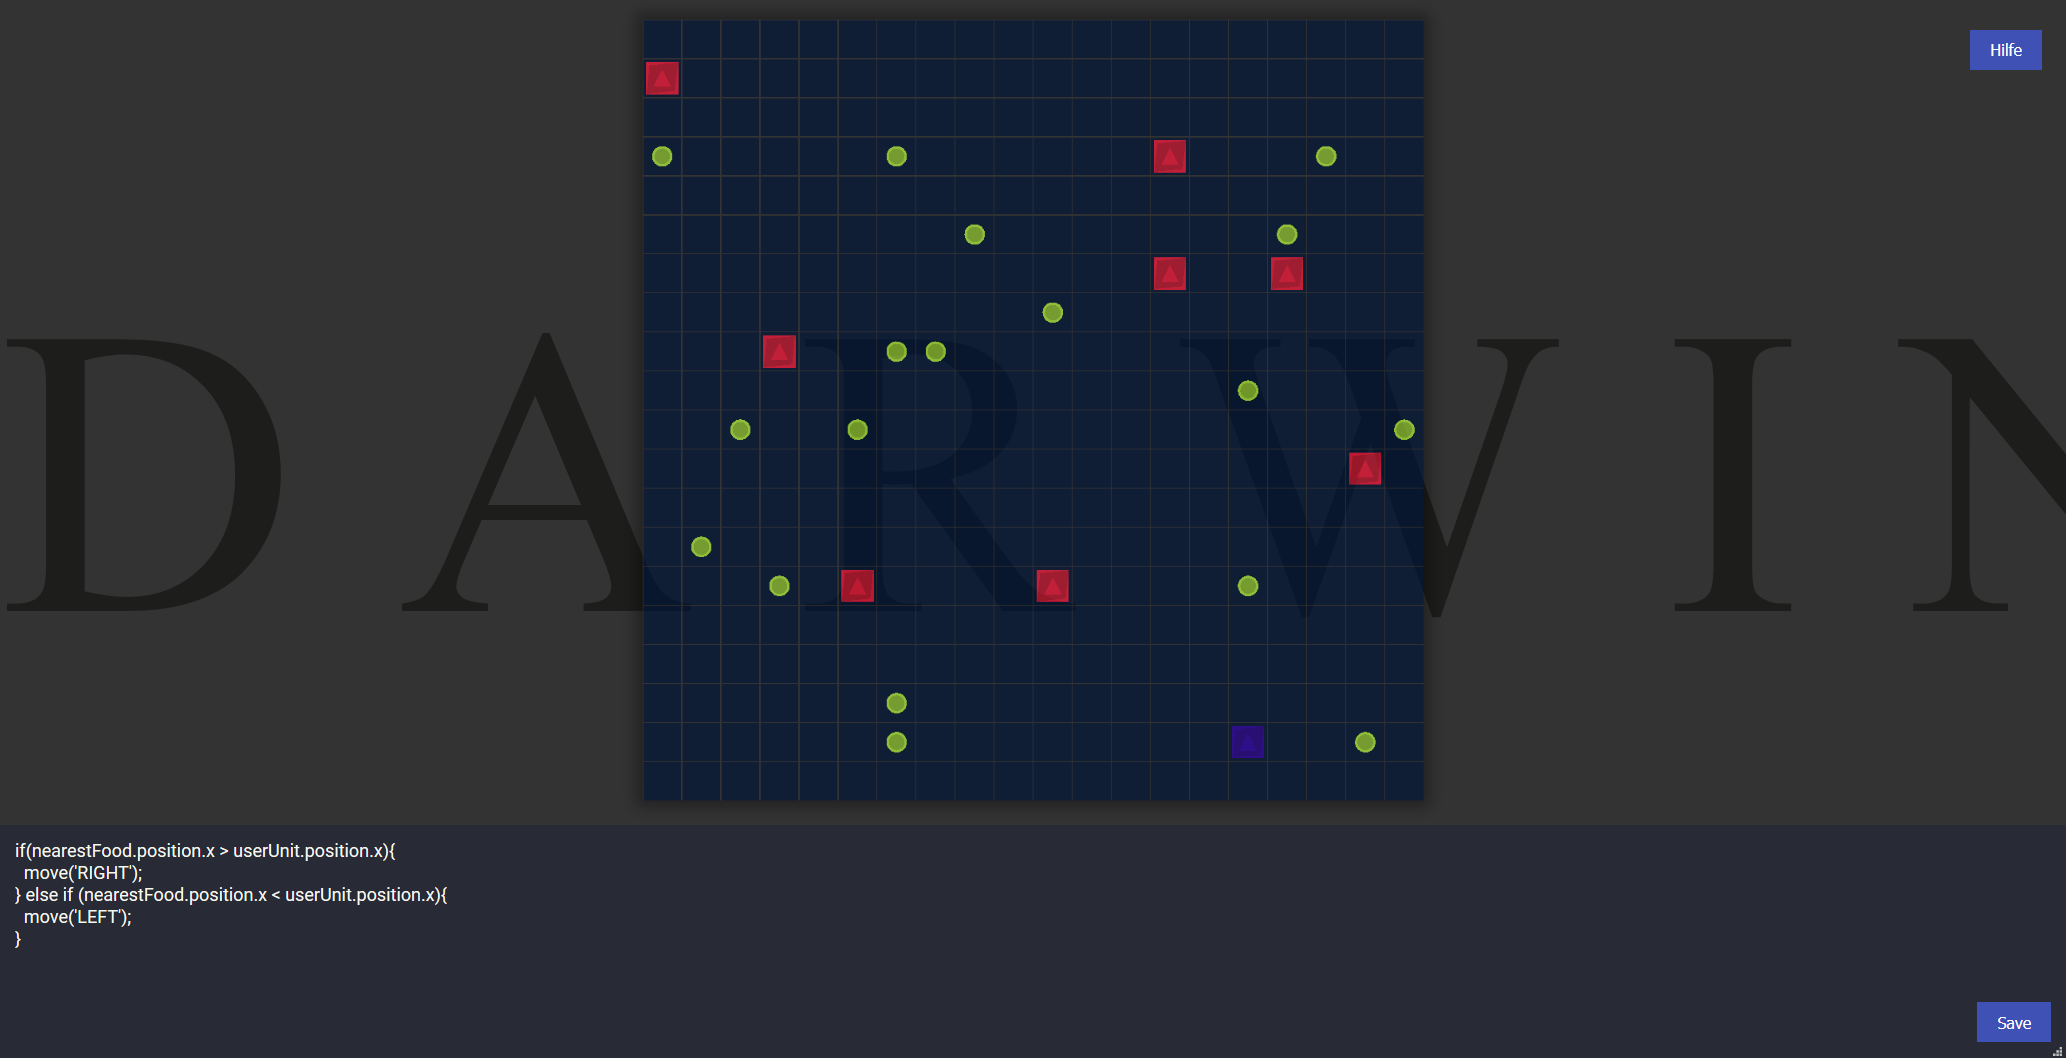
\includegraphics[width=\textwidth]{darwin-gameplay.png}


\subsection{Spielfeld}

Das Spielfeld besteht aus kleinen Quadraten, die entweder leer oder mit geometrischen Figuren gefüllt sind. Die geometrischen Formen haben folgende Bedeutung:
\begin{itemize}
\item Grünes Quadrat: Der aktuelle Spieler ("ich")
\item Rotes Quadrat: Anderer Spieler ("Gegner")
\item Balken über den Quadraten: Gesundheitszustand der Spieler ("Health")
\item Blauer Kreis: Nahrung
\item Kleine Quadrate (verschiedene Farben): "Power-Ups"
\end{itemize}

Die Darstellung der Icons auf dem Spielfeld wurde zu Beginn etwas aufwändiger geplant, jedoch bald verworfen. Die komplexe Darstellung hätte zwar ein historisches Thema ins Spiel gebracht, jedoch inhaltlich keinen Mehrwert geliefert. Die jetzt verwendeten geometrischen Formen sind sehr klar, für den Spieler gut erkennbar und passen auch insgesamt gut zur Grafik. Wir sind deshalb mit dieser Anpassung zufrieden.

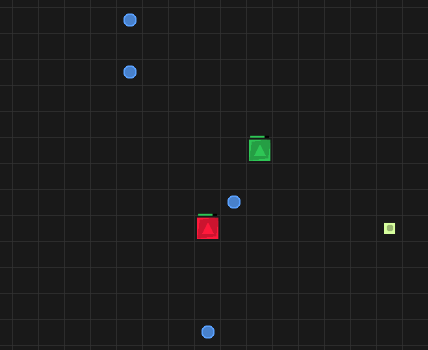
\includegraphics[width=\textwidth]{game1.png}

\subsection{Spielführung}

Gespielt wird mittels Eingabe von Code, z.B. \texttt{move('LEFT')}. Ziel ist es, als letzter zu überleben. Um am Leben zu bleiben, muss man Nahrung aufsammeln und konsumieren. Man kann sich Vorteile verschaffen durch das Konsumieren von Power-Ups. Bewegt man sich auf ein Feld auf dem der andere Spieler sich befindet, attackiert man diesen.

Die Regeln des Spiels sind sehr einfach gehalten, damit kann sich der Spieler auf das Wesentliche konzentieren, nämlich das Coden zu erlernen und seine Strategie in Code umzusetzen.

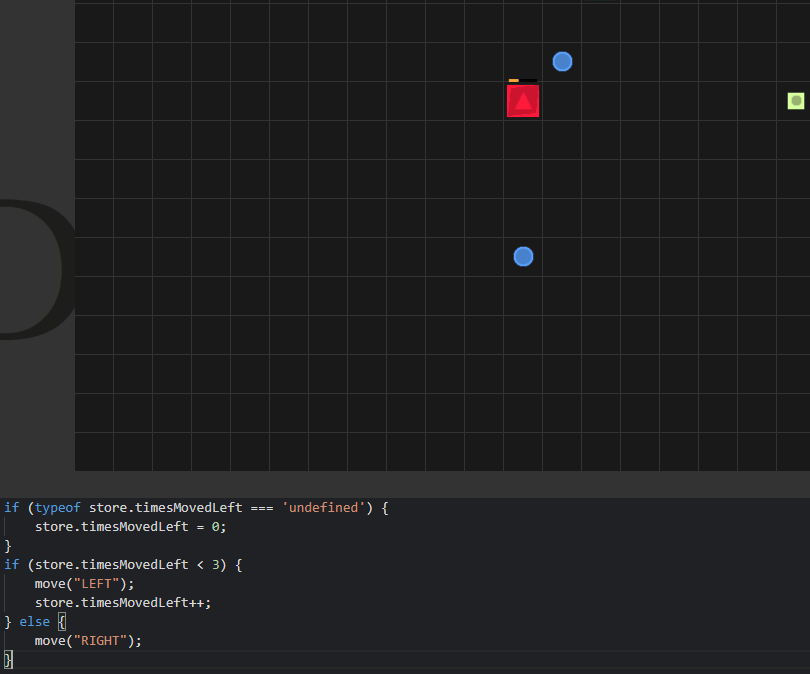
\includegraphics[width=\textwidth]{game2.png}

\subsection{Ausblick}

Es gibt diverse Erweiterungsmöglichkeiten für das Spiel. Einige sind im Folgenden näher beschrieben:

\subsubsection{UI}
Wir könnten uns überlegen, das ursprünglich angedachte, komplexere Iconset zu implementieren. Der Spieler könnte sich damit vielleicht besser mit der Story identifizieren. Dies hat für uns allerdings im Moment keine Priorität.

\subsubsection{Befehlsset}
In Zukunft könnten die zur Verfügung stehenden Kommandos erweitert werden, z.B. durch weiterführende Levels, so dass auch neue Strategien möglich werden. Damit könnte man z.B. die Spieler durch verschiedene Lernstufen begleiten und sie würden ihr Können Schritt für Schritt verbessern.

\subsubsection{Spielmodus}
Wir könnten uns vorstellen, verschiedene neue Gems mit neuen Bedeutungen einzuführen die man sammeln kann oder denen man z.B. auch ausweichen muss. Dies könnte das Spiel aber unnötig verkomplizieren ohne, dass der Spieler seine Programmierfährigkeiten notwendigerweise verbessert. Daher müssen wir diese Anpassungen sehr vorsichtig vornehmen.

\section{Literaturverzeichnis}
%Beispiele Grundmuster Harvard-System:
%Deutsch:\\
%Name, Vorname (Jahreszahl): \textit{Titel. Unertitel.} ev. Vorname Name (Hrsg.), ev. Bd., ev. Auflage. Verlagsort: Verlag 
%Englisch:\\
%Author surname, Initials. (Year). title. ed. City: Publisher, p.Pages Used.

\begin{itemize}
\item [1] Wikipedia, Type Script [online]. URL: https://de.wikipedia.org/wiki/TypeScript (Abgerufen am 18.04.2020).
\item [2] Entwickler Onlinemagazin.  [online]. \\URL: https://entwickler.de/online/javascript/7-gruende-node-js-579924149.html (Abgerufen am 18.04.2020).
\item [3] React Handbook [online]. \\URL: https://www.freecodecamp.org/news/the-react-handbook-b71c27b0a795/ (Abgerufen am 18.04.2020).
\item [4] Lerna. URL: https://lerna.js.org/ (Abgerufen am 18.04.2020).
\end{itemize}

\end{document}